\documentclass[12pt]{article}
% Geometria i fonty jak w szablonie prowadzacego: letterpaper, 12pt, bez geometry.
\usepackage{iftex}
\ifPDFTeX
  \usepackage[utf8]{inputenc}
\else
  \usepackage{fontspec}
  \setmainfont{lmroman10-regular.otf}[
    BoldFont       = lmroman10-bold.otf,
    ItalicFont     = lmroman10-italic.otf,
    BoldItalicFont = lmroman10-bolditalic.otf]
\fi
\usepackage[polish]{babel}
\usepackage{amsmath,amssymb}
\usepackage{booktabs}
\usepackage{graphicx}
\usepackage{caption}
\addto\captionspolish{\renewcommand{\refname}{Bibliografia}}

\title{\textbf{Zadanie nr 2 - sieć MADALINE do rozpoznawania znaków}\\[2mm]
       \large Inteligentna Analiza Danych}
\author{Łukasz Centkowski 264303 \\ Maciej Dominiak 264307}
\date{25 października 2026}

\begin{document}
\maketitle
\thispagestyle{empty}
\newpage

\section{Cel zadania}

Zadanie polegało na zbudowaniu sieci MADALINE rozpoznającej znaki graficzne.
Wzorce znaków sieć wczytuje z~plików obrazowych. Sprawdziliśmy, do jakiego
poziomu zaszumienia rozpoznawanie działa poprawnie i~od czego ta granica zależy.

\section{Wstęp teoretyczny}

Neuron liniowy liczy iloczyn skalarny swoich wag i~wejścia. Gdy oba wektory mają
długość jeden, wynik jest cosinusem kąta między nimi, czyli liczbą z~przedziału
$[0,1]$ mówiącą, jak bardzo są do siebie podobne~\cite{wyklad}.

Sieć MADALINE opiera się na tej własności. Ma jedną warstwę neuronów liniowych
i~każdy neuron odpowiada za jeden znak wzorcowy. Wszystkie neurony dostają to
samo wejście, a~wygrywa ten o~największym wyjściu~\cite{widrow,osowski}.

Wagi neuronu ustawiamy po prostu na znormalizowany wzorzec jego znaku, więc
\emph{nie ma tu żadnego treningu}. Obraz zamieniamy na wektor w~trzech krokach:
binaryzacja, sklejenie wierszy jeden za drugim, podzielenie przez długość. Tusz
koduje jedynka, tło zero. Przy odwrotnej konwencji wszystkie podobieństwa
wyszłyby bliskie jedności, bo tło zajmuje ponad $90\%$ obrazu.

Podobieństwo wzorca do jego zaszumionej wersji można przewidzieć. Niech wzorzec
ma $n$ pikseli tuszu, obraz $P$~pikseli, a~każdy piksel odwraca się
z~prawdopodobieństwem $p$. Wspólnych pikseli tuszu zostaje średnio $(1-p)\,n$,
a~z~tła dochodzi $p\,(P-n)$ nowych. Stąd
\begin{equation}
\cos \;=\; \frac{(1-p)\,n}{\sqrt{n}\,\sqrt{(1-p)\,n + p\,(P-n)}}\,.
\label{eq:model}
\end{equation}

\section{Eksperymenty i wyniki}

Implementacja to dwa programy konsolowe. \texttt{font\_generator.py} rysuje
literę i~zaszumia ją, a~\texttt{madaline\_ocr.py} buduje sieć ze wzorców
w~jednym katalogu i~rozpoznaje znaki z~drugiego. Plik \texttt{description.txt}
wiąże nazwy obrazów z~etykietami znaków. Użyliśmy liter \texttt{a}, \texttt{b}
i~\texttt{c} w~kroju Times New Roman, na obrazach $128\times128$ pikseli.

\subsection{Eksperyment nr 1: weryfikacja wobec przykładu z wykładu}

\subsubsection{Założenia}
Materiały do wykładu podają gotowe wyniki dla kształtów $4\times4$ liter
X,~Y,~Z oraz zaburzonej litery~X. Można więc sprawdzić implementację na
wartościach znanych z~góry, bez udziału generowanych obrazów.

\subsubsection{Przebieg}
Trzem neuronom przypisaliśmy znormalizowane kształty liter X,~Y i~Z. Na wejście
podaliśmy zaburzoną literę~X, która różni się od wzorca jednym pikselem.

\subsubsection{Rezultat}
Porównanie zawiera Tab.~\ref{tab:wyklad}.

\begin{table}[h]
\centering
\caption{Stopnie podobieństwa dla kształtów $4\times4$ z~materiałów wykładowych}
\label{tab:wyklad}
\begin{tabular}{lcc}
\toprule
\textbf{Wzorzec oryginalny} & \textbf{Materiały} & \textbf{Implementacja} \\
\midrule
litera X & 0,943 & 0,943 \\
litera Y & 0,816 & 0,816 \\
litera Z & 0,738 & 0,738 \\
\bottomrule
\end{tabular}
\end{table}

Wszystkie trzy wartości zgadzają się co do trzeciego miejsca po przecinku.
Normalizacja wektorów i~liczenie podobieństwa działają więc poprawnie.

\subsection{Eksperyment nr 2: rozpoznawanie znaków zaszumionych}

\subsubsection{Założenia}
Wzorce wygenerowaliśmy bez szumu, a~znaki testowe przy pięciu poziomach: $0$,
$10$, $30$, $50$ i~$90\%$. Poziom to prawdopodobieństwo odwrócenia jednego
piksela. Szum dotyczy zarówno tuszu, jak i~tła.

\subsubsection{Przebieg}
Sieć zbudowaliśmy ze wzorców bez szumu. Potem rozpoznawaliśmy kolejne zestawy
znaków testowych i~zapisywaliśmy wskazanie sieci oraz podobieństwo do
zwycięskiego wzorca. Jak wyglądają znaki testowe, pokazuje Rys.~\ref{fig:wzorce}.

\begin{figure}[htbp]
\centering
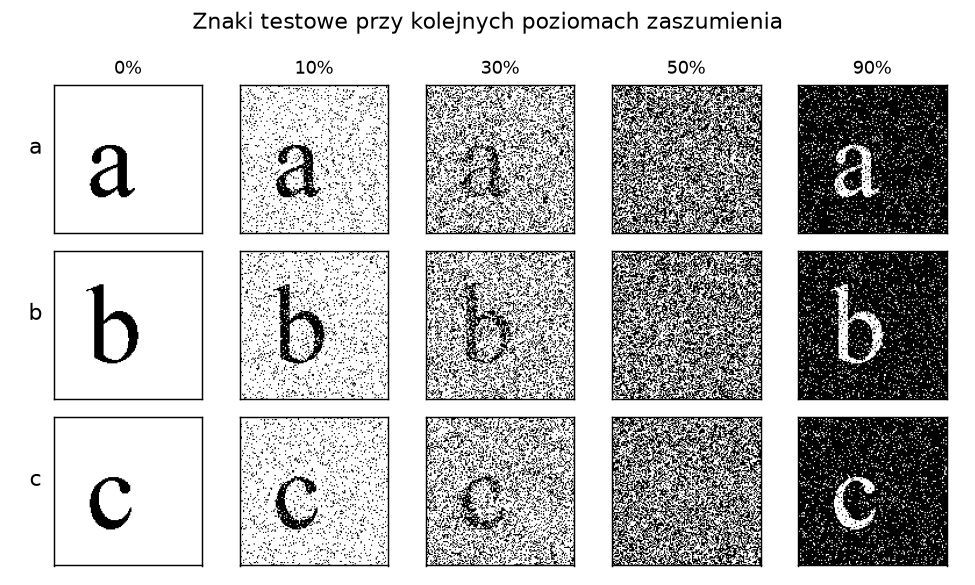
\includegraphics[width=0.85\textwidth]{wyniki/wzorce_szum.png}
\caption{Znaki testowe przy kolejnych poziomach zaszumienia}
\label{fig:wzorce}
\end{figure}

\subsubsection{Rezultat}
Wyniki zestawiono w~Tab.~\ref{tab:szum}; wytłuszczono wskazania błędne.

\begin{table}[h]
\centering
\caption{Rozpoznawanie znaków przy rosnącym zaszumieniu}
\label{tab:szum}
\begin{tabular}{ccccc}
\toprule
\textbf{Poziom szumu} & \textbf{a} $\rightarrow$ & \textbf{b} $\rightarrow$ &
\textbf{c} $\rightarrow$ & \textbf{Poprawnie} \\
\midrule
0\%  & a (1,000)          & b (1,000)          & c (1,000)          & 3/3 \\
10\% & a (0,522)          & b (0,577)          & c (0,489)          & 3/3 \\
30\% & a (0,264)          & b (0,303)          & c (0,244)          & 3/3 \\
50\% & \textbf{b} (0,170) & b (0,174)          & \textbf{b} (0,167) & 1/3 \\
90\% & \textbf{b} (0,170) & \textbf{a} (0,128) & \textbf{b} (0,153) & 0/3 \\
\bottomrule
\end{tabular}
\end{table}

Do $30\%$ zaszumienia sieć nie myli się ani razu. Przy $50\%$ rozpoznaje
poprawnie jeden znak na trzy, a~przy $90\%$ żadnego. Uwagę zwraca szybki spadek
podobieństwa: przy $10\%$ szumu wynosi ono już tylko około $0{,}5$, choć
człowiek nadal czyta literę bez trudu, co widać na Rys.~\ref{fig:wzorce}.

Przy $50\%$ i~$90\%$ sieć wskazuje niemal zawsze literę \texttt{b}, bez względu
na to, co jest na obrazie.

\subsection{Eksperyment nr 3: przyczyna spadku stopnia podobieństwa}

\subsubsection{Założenia}
Chcieliśmy ustalić dwie rzeczy. Po pierwsze, czy szybki spadek podobieństwa to
cecha metody, czy błąd w~kodzie. Po drugie, dlaczego przy dużym szumie wygrywa
zawsze ten sam neuron. Postawiliśmy hipotezę, że decyduje udział tuszu
w~powierzchni obrazu.

\subsubsection{Przebieg}
Policzyliśmy piksele tuszu każdego wzorca i~porównaliśmy zmierzone wyjście
neuronu danej litery z~wartością ze wzoru~(\ref{eq:model}). Porównujemy wyjście
neuronu \emph{właściwej} litery, a~nie zwycięskiego, bo powyżej $30\%$ szumu
wygrywa już neuron innej litery.

\subsubsection{Rezultat}
Udział tuszu zestawia Tab.~\ref{tab:tusz}, a~porównanie z~modelem
Tab.~\ref{tab:model} oraz Rys.~\ref{fig:pewnosc}.

\begin{table}[h]
\centering
\caption{Udział pikseli tuszu w~powierzchni obrazu}
\label{tab:tusz}
\begin{tabular}{lccc}
\toprule
\textbf{Wzorzec} & \textbf{Piksele tuszu} & \textbf{Piksele ogółem} & \textbf{Udział} \\
\midrule
litera a & 761 & 16384 & 4,6\% \\
litera b & 999 & 16384 & 6,1\% \\
litera c & 609 & 16384 & 3,7\% \\
\bottomrule
\end{tabular}
\end{table}

\begin{table}[h]
\centering
\caption{Wyjście neuronu właściwej litery kontra model~(\ref{eq:model})}
\label{tab:model}
\small
\begin{tabular}{lcccccc}
\toprule
 & \multicolumn{5}{c}{\textbf{Poziom zaszumienia}} \\
\cmidrule(l){2-6}
\textbf{Wzorzec} & 0\% & 10\% & 30\% & 50\% & 90\% \\
\midrule
litera a, pomiar & 1,000 & 0,522 & 0,264 & 0,138 & 0,026 \\
litera a, model  & 1,000 & 0,524 & 0,267 & 0,152 & 0,023 \\[1mm]
litera b, pomiar & 1,000 & 0,577 & 0,303 & 0,174 & 0,027 \\
litera b, model  & 1,000 & 0,576 & 0,303 & 0,175 & 0,027 \\[1mm]
litera c, pomiar & 1,000 & 0,489 & 0,244 & 0,130 & 0,016 \\
litera c, model  & 1,000 & 0,482 & 0,241 & 0,136 & 0,021 \\
\bottomrule
\end{tabular}
\end{table}

\begin{figure}[htbp]
\centering
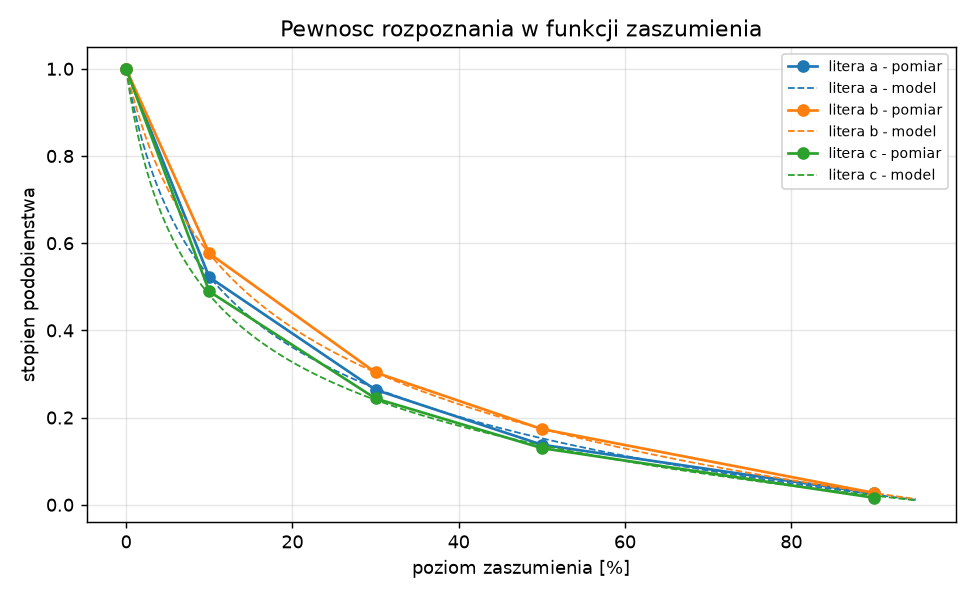
\includegraphics[width=0.9\textwidth]{wyniki/pewnosc_szum.png}
\caption{Zmierzony stopień podobieństwa i~krzywa modelu~(\ref{eq:model})}
\label{fig:pewnosc}
\end{figure}

Model trafia w~pomiar na całym zakresie, z~różnicą najwyżej $0{,}015$. Spadek
podobieństwa jest więc cechą metody, a~nie błędem w~kodzie. Przyczynę widać we
wzorze~(\ref{eq:model}). Litera zajmuje kilka procent obrazu, więc przy $10\%$
szumu z~tła dochodzi około $1560$ losowych pikseli tuszu, czyli \emph{dwa razy
więcej}, niż ma sama litera. Mianownik rośnie wtedy dużo szybciej, niż maleje
licznik.

Tabela~\ref{tab:tusz} tłumaczy też przewagę litery \texttt{b} przy dużym szumie.
Dla wejścia bliskiego losowemu średni iloczyn skalarny z~neuronem $i$ rośnie jak
$\sqrt{n_i}$, więc wygrywa neuron o~najliczniejszym wzorcu. Litera \texttt{b} ma
$999$ pikseli tuszu, a~pozostałe $761$ i~$609$. Dlatego wygrywa niezależnie od
tego, co jest na obrazie.

\section{Wnioski}

\paragraph{Poprawność i~odporność na szum.} Dla kształtów $4\times4$
z~materiałów wykładowych nasza implementacja zwraca te same wartości co do
trzeciego miejsca po przecinku. Wzorce bez szumu rozpoznaje z~podobieństwem
równym dokładnie $1{,}000$. Rozpoznawanie jest bezbłędne do $30\%$ zaszumienia.
Przy $50\%$ poprawny jest jeden znak na trzy, a~przy $90\%$ żaden.

\paragraph{Jak czytać stopień podobieństwa.} To nie jest prawdopodobieństwo,
tylko cosinus kąta. Spadek do około $0{,}5$ przy $10\%$ szumu nie znaczy, że
sieć „prawie się myli''. Znak jest wtedy rozpoznawany pewnie, a~przewaga nad
pozostałymi wzorcami pozostaje wyraźna. Niska wartość bierze się stąd, że szum
dotyka całego obrazu, a~litera zajmuje kilka procent jego powierzchni.
Skuteczność zależy więc nie tylko od poziomu szumu, ale też od proporcji tuszu
do tła. W~praktyce znaczy to tyle, że obraz warto kadrować ciasno wokół znaku.

\paragraph{Brak mechanizmu odrzucenia.} Sieć MADALINE zawsze wskazuje jakiegoś
zwycięzcę, nawet gdy na wejściu nie ma żadnego znaku. Przy dużym szumie wskazuje
po prostu wzorzec o~największej powierzchni, co pokazał eksperyment nr~3. Praktyczny system rozpoznawania znaków wymagałby progu odrzucenia opartego na
stopniu podobieństwa. Dla badanego zestawu próg taki musi leżeć między $0{,}174$,
czyli najwyższą wartością towarzyszącą wskazaniu błędnemu, a~$0{,}244$, czyli
najniższą towarzyszącą wskazaniu poprawnemu; wartość $0{,}2$ oddziela te dwa
zbiory w~całym przebadanym zakresie zaszumienia.

\section{Załączniki}

Rdzeń implementacji: wektor wagowy każdego neuronu ustawiany wprost na
znormalizowany wzorzec, bez treningu iteracyjnego (plik \texttt{madaline.py}).

\begin{verbatim}
network = Network([len(vectors[0]), len(vectors)], bias=False,
                  activations=[(linear, linear_derivative)])
for neuron, vector in zip(network.layer_list[0].neurons, vectors):
    neuron.weights = vector
\end{verbatim}

\begin{thebibliography}{9}

\bibitem{wyklad}
K. Stokfiszewski.
\textit{Inteligentna Analiza Danych. Materiały do wykładu nr 1 i~nr 2}.
Instytut Informatyki Politechniki Łódzkiej.

\bibitem{widrow}
B. Widrow, M. E. Hoff.
\textit{Adaptive switching circuits}.
IRE WESCON Convention Record, 1960.

\bibitem{osowski}
S. Osowski.
\textit{Sieci neuronowe do przetwarzania informacji}.
Oficyna Wydawnicza Politechniki Warszawskiej, Warszawa.

\end{thebibliography}

\end{document}
